% THIS IS SIGPROC-SP.TEX - VERSION 3.1
% WORKS WITH V3.2SP OF ACM_PROC_ARTICLE-SP.CLS
% APRIL 2009
%
% It is an example file showing how to use the 'acm_proc_article-sp.cls' V3.2SP
% LaTeX2e document class file for Conference Proceedings submissions.
% ----------------------------------------------------------------------------------------------------------------
% This .tex file (and associated .cls V3.2SP) *DOES NOT* produce:
%       1) The Permission Statement
%       2) The Conference (location) Info information
%       3) The Copyright Line with ACM data
%       4) Page numbering
% ---------------------------------------------------------------------------------------------------------------
% It is an example which *does* use the .bib file (from which the .bbl file
% is produced).
% REMEMBER HOWEVER: After having produced the .bbl file,
% and prior to final submission,
% you need to 'insert'  your .bbl file into your source .tex file so as to provide
% ONE 'self-contained' source file.
%
% Questions regarding SIGS should be sent to
% Adrienne Griscti ---> griscti@acm.org
%
% Questions/suggestions regarding the guidelines, .tex and .cls files, etc. to
% Gerald Murray ---> murray@hq.acm.org
%
% For tracking purposes - this is V3.1SP - APRIL 2009

\documentclass{acm_proc_article-sp}
% these seem necessary to get 8.5x11 (letter) page size working in pdflatex
\setlength{\pdfpagewidth}{8.5in}
\setlength{\pdfpageheight}{11in}
\usepackage[export]{adjustbox}
\usepackage{minted}
\usepackage{caption}
\usepackage{tikz}

\usemintedstyle{friendly}
\newminted{json}{linenos=false, stepnumber=1, frame=lines, framesep=1em}

\newenvironment{tightitemize}{
    \vspace{-10pt}
    \begin{itemize}
        \setlength{\parskip}{-1pt}}{
    \end{itemize}
    \vspace{-10pt}}

\newenvironment{tightenumerate}{
    \vspace{-10pt}
    \begin{enumerate}
        \setlength{\parskip}{-1pt}}{
    \end{enumerate}
    \vspace{-10pt}}

% command from http://www.acm.org/sigs/publications/sigfaq
\def\sharedaffiliation{
\end{tabular}
\begin{tabular}{c}}

\begin{document}

\title{Hypermedia APIs for Sensor Data}
\subtitle{A pragmatic approach to the Web of Things}
\toappear{Submitted to 11th International Conference on Mobile and Ubiquitous
    Systems: Computing, Networking and Services (Mobiquitous 2014)\\
    December 2-5, 2014\\
    London, Great Britain}

% You need the command \numberofauthors to handle the 'placement
% and alignment' of the authors beneath the title.
%
% For aesthetic reasons, we recommend 'three authors at a time'
% i.e. three 'name/affiliation blocks' be placed beneath the title.
%
% NOTE: You are NOT restricted in how many 'rows' of
% "name/affiliations" may appear. We just ask that you restrict
% the number of 'columns' to three.
%
% Because of the available 'opening page real-estate'
% we ask you to refrain from putting more than six authors
% (two rows with three columns) beneath the article title.
% More than six makes the first-page appear very cluttered indeed.
%
% Use the \alignauthor commands to handle the names
% and affiliations for an 'aesthetic maximum' of six authors.
% Add names, affiliations, addresses for
% the seventh etc. author(s) as the argument for the
% \additionalauthors command.
% These 'additional authors' will be output/set for you
% without further effort on your part as the last section in
% the body of your article BEFORE References or any Appendices.

\numberofauthors{2}

%\author{
% You can go ahead and credit any number of authors here,
% e.g. one 'row of three' or two rows (consisting of one row of three
% and a second row of one, two or three).
%
% The command \alignauthor (no curly braces needed) should
% precede each author name, affiliation/snail-mail address and
% e-mail address. Additionally, tag each line of
% affiliation/address with \affaddr, and tag the
% e-mail address with \email.
%
% 1st. author
%\alignauthor Spencer Russell\\
%    \email{sfr@media.mit.edu}
%% 2nd. author
%\alignauthor Joseph A. Paradiso\\
%    \email{joep@media.mit.edu}
%\sharedaffiliation
%    \\
%    \affaddr{Responsive Environments Group}  \\
%    \affaddr{MIT Media Lab}   \\
%    \affaddr{Massachusetts Institute of Technology} \\
%    \affaddr{Cambridge, MA, USA}
%}

\author{
% 1st. author
\alignauthor Author One\\
    \email{author1@example.com}
% 2nd. author
\alignauthor Author Two\\
    \email{author2@example.com}
\sharedaffiliation
    \\
    \affaddr{Research Group}  \\
    \affaddr{Research Institution} \\
    \affaddr{Research Location}
}

\date{14 July 2014}

\maketitle

\begin{abstract}
As infrastructure for the Internet of Things becomes more commonplace, an
application layer is needed to enable interoperability and create a \emph{Web}
of Things. Here we introduce a pragmatic approach to the Web of Things that is
inspired equally by the rich body of Semantic Web research and industry web
services practice. This approach integrates HTTP request/response interactions
with realtime streaming using HTML5 WebSockets. We will discuss how our
approach enables client/server interactions that are both evolvable by the
server and discoverable by the client. Rather than attempt to define yet
another competing standard, we incorporate a collection of complementary
standards already in use. We will also describe our implementation of these
concepts in ChainAPI, a sensor data server in use by a variety of projects at
\emph{REDACTED}. We have developed several end-to-end applications with this
infrastructure, and we will describe two of them as successful case studies.
\end{abstract}


% % A category with the (minimum) three required fields
% \category{H.4}{Information Systems Applications}{Miscellaneous}
% %A category including the fourth, optional field follows...
% \category{D.2.8}{Software Engineering}{Metrics}[complexity measures, performance measures]
%
% \terms{Theory}
%
\keywords{Semantic Web, RESTful Web Services, Sensors, Internet of Things, Hypermedia} % NOT required for Proceedings

\section{Introduction}

It is becoming apparent that in addition to a transport layer that enables the
so-called Internet of Things, it is important to develop an application layer
to provide wide-spread interoperability and a consistent interface to
internet-connected devices. While there are many efforts [cite Alljoyn, etc.]
to develop new standards and protocols, other projects [cite] seek to use
existing application-level web standards such as HTTP to provide an interface
that is more familiar to developers, and also that can take advantage of
tooling and infrastructure already in place for the World Wide Web. Reflecting
the relationships to existing web standards and also the way in which the World
Wide Web is built on top of the Internet, these efforts are often dubbed the
Web of Things.

In previous work~\cite{doppellab}\cite{gestures} we have built frameworks to collect
and process sensor data from a variety of sources, as well as applications to
visualize and experience those data. [Expand on how this informed ChainAPI]

We posit that the main impediments to adoption of IoT standards are social
rather then technological. Often  solutions require developers to take on too much
simultaneous complexity to get started. Many of the systems coming from a Semantic
Web history have sophisticated data models to ensure compatibility with existing
upper ontologies [cite]. Application developers are often unwillinging to adopt
this additional complexity [why?].

To address these issues we have developed and implemented an API that interoperates
easily with existing infrastructure, and also allows developers to take advantage
of semantic relations and formal ontologies without requiring it.

\section{Related Work}

What are other approaches? Alljoyn? Semantic-web approaches in SPARQL
databases?

\section{Hypermedia Web Services}

One of the most influential works in Hypermedia Web Services is Roy Fielding's
PhD dissertation ``Architectural Styles and the Design of Network-based
Software Architectures''~\cite{fielding}. Fielding codified much of the design
that had gone into the World Wide Web into an architectural framework he called
Representational State Transfer, or REST. He lists the main requirements that
drove the design of the World Wide Web:

\begin{tightitemize}
    \item Low barrier to entry
    \item Extensibility
    \item Distributed hypermedia
    \item Internet-scale
\end{tightitemize}

The Internet of Things certainly must be extensible and Internet-Scale. This work
focuses on exploring the benefits of lowering barriers to entry and hypermedia.

\section{Bringing Poll and Push\\ Together}

In ChainAPI we focus on integrating request/response interactions with realtime
push or pub/sub updates. Many interactions map well to a Hypermedia HTTP API in
which clients make a request and the server sends a response, there is abundant
tooling and library support, and it is a simple and well-defined exchange
between client and server. However, it is very common in sensor data systems to
want new sensor data as soon as it is available, a task that HTTP is not
particularly well suited for. While many workarounds such as long-polling are
in common use, HTML5 WebSockets are intended for just this use case.

Clients begin interacting with ChainAPI via the Hypermedia HTTP API, by submitting
HTTP requests for resources and receiving responses with representations of
those resources in HAL+json. While browsing the available resources, the server
may wish to provide a realtime feed for related data. In our system the server
can communicate that the stream is available simply by providing a
\texttt{ch:websocketStream} link relation. For example, in Listing
\ref{sensorjson} the server is telling the client that there is a WebSocket
stream for this sensor available at \texttt{ws://example.com/ws/sensor-274}. As
new data from the sensor is available it will be streamed to all subscribed
clients. Because there is a natural hierarchy in our data (many devices in a
Site, usually several sensors in each Device), when clients subscribe to a resource
they get updates for all resources below them in the hierarchy.

\begin{listing}
\begin{jsoncode}
  {
    "updated": "2014-04-01T02:34:21.676564+00:00",
    "dataType": "float",
    "metric": "sht_temperature",
    "value": 25.59,
    "_links": {
      "ch:dataHistory": {
        "href": "/sensordata/?sensor_id=274",
        "title": "Data"
      },
      "curies": [
        {
          "href": "/rels/{rel}",
          "name": "ch",
          "templated": true
        }
      ],
      "self": {
        "href": "/sensors/274"
      },
      "ch:device": {
        "href": "/devices/33",
        "title": "Office Thermostat"
      },
      "ch:websocketStream": {
        "href": "ws://example.com/ws/sensor-274",
        "title": "Websocket Stream"
      },
      "editForm": {
        "href": "/sensors/274/edit",
        "title": "Edit Sensor"
      }
    },
    "unit": "celsius"
  }
\end{jsoncode}
\caption{hal+json representation of a sensor}
\label{sensorjson}
\end{listing}


\section{Layered Architecture}

Work is under way by multiple groups to adapt the TCP/IP Stack to be more
suitable for low-power, resource-constrained devices~\cite{iotsurvey}.  Though
this is a reasonable proposition and would provide a suitable transport
protocol for communication, it leaves open many questions that are important
for secure and reliable communication over the open internet. Even if the
devices themselves speak IP (whether using WiFi, 6LoWPAN, etc.) there will
still likely be a role for a bridge or gateway node that can handle encryption,
authentication, discovery mechanisms, and other application logic necessary to
communicate and interoperate with the larger Internet.

One of the benefits of this approach is that we can take advantage of existing
HTTP Caching and Proxy infrastructure. It is a common pattern in modern web
development to have application web server processes handling application
logic, and to place a front-end HTTP server such as Nginx or Apache as a proxy.
In this configuration, the proxy is responsible for handling SSL, defending
against DDOS attacks, and in general provides a front line of defense to the
open internet. The application server processes (e.g. Node.js or Gunicorn) thus
operate in a safer environment and focus on handling application logic.

This layered architecture has been used in Web of Things literature to
divide direct from indirect integration~\cite{wotsurvey}. In direct
integration, the devices themselves are capable of serving requests directly
from clients. In indirect integration there is a gateway or bridge that serves
the requests, and translates them to a protocol that the (presumably
lower-powered) nodes can understand. An unexplored middle ground is for end
devices to function as simple HTTP servers that are proxied behind more complex
ones. For example, a gateway could handle SSL and authentication, but then
forward requests to the simpler devices for handling application logic. This
layered architecture is one of the six constraints that define the REST
architecture~\cite{fielding}.

The standard HTTP methods (\texttt{GET}, \texttt{POST}, etc.) have well-defined
semantics~\cite{httpmethods}. For instance, a \texttt{GET} request should have
no side effects in the server, and a \texttt{PUT} request should be idempotent
(making the request more than once has the same effect as making it once, i.e.
the request can be safely repeated). Using these standard methods and adhering
to the defined semantics allows intermediate servers to behave more
intelligently and route traffic more effeciently. One notable example is the
caching proxy.  There exist many widely-used proxies such as
Varnish\footnote{https://www.varnish-cache.org/},
Nginx\footnote{http://nginx.org/}, and
Squid\footnote{http://www.squid-cache.org/} that can take advantage of the HTTP
method along with standardized cache lifetime HTTP headers to intercept the
request and serve a cached response from a previous request, reducing the load
on the application server, which might otherwise have needed to access a
database or do other expensive calculations to re-build the response.

\section{Enabling Search}

In the early days of the World Wide Web, sites were primarily accessed directly
via their URLs, or via links from other known sites. In the earliest days in
fact, CERN had an alphabatized index of available web
content~\cite{websearchengines}. As the web grew beyond what could be
reasonably browsed and bookmarked, the problem of finding information on the
Web changed. It was no longer enough for the content to be on the web, it also
had to be discoverable in a sea of other pages. By 1994 search engines started
to appear to allow users to find the information they wanted. With search
engines came the advent of crawlers that would index the web and collect the
metadata into the engine's database. As more sensors and sensor networks are
added to the Web of Things, similar issues will arise. Our approach can serve
as a substrate on which a similar ecosystem of crawlers can index the available
data and metadata.

\section{Naming}

One of the central issues in the IoT is simply the issue of uniquely
identifying objects in the system~\cite{iotsurvey}. We propose the use of HTTP
URIs as globally unique identifiers.  Providers can structure their URIs
aritrarily, for instance to represent natural hierarchy in the system. Link
relations between objects not only represent identity, but also where the
linked object can be found, without needing to first consult any sort of
central registry.

Additionally, HTTP has built-in mechanisms to handle renaming, as servers can
respond with an HTTP Status 301 (Moved Permanently) to notify clients that the
object can now be found at a new URI.

\section{Using Existing Standards}

Wherever possible we have relied on existing standards and protocols rather
than reinventing our own. For instance, to support hypermedia in our responses
we are using the Hypertext Application Language~\cite{json-hal-draft}, which
provides a standardized data model for hyperlinks that can be rendered in JSON
or XML (though JSON is the main focus and was implemented by the authors).

Hal+json provides a mechanism for the server to present affordances to the
client in the form of links. For requesting those resources the client simply
issues an HTTP \texttt{GET} request to the given URL. Actions such as posting
new sensor data or adding a new sensor require the client to send data to the
server. The client can send data to the server via \texttt{POST} requests with
data encoded in the body of the request with JSON. The server can provide the
client with the expected format of the data using
JSON-Schema~\cite{json-schema-draft}. We use the IANA-standardized link
relations \texttt{edit-form} and \texttt{create-form} to indicate link
relations that can be used for editing and creating resources. A \texttt{GET}
request to the given relation will generate a response with the expected
schema, and a \texttt{POST} will edit or create the resource, depending on the
relation.

\section{Supporting a Relation Ontology}

ChainAPI is inspired by the rich literature and history of the Semantic Web.
This section needs to talk about how our links can support various ontologies,
and talk a little about ours.

\section{API Description}

To validate our design choices and experiment in a real-world environment, we
have implemented a server-side web service called ChainAPI. We have also
created several client applications to use the service in different ways.

ChainAPI is released under the MIT license, and source code is available on
GitHub\footnote{https://github.com/ssfrr/chain-api}.

\subsection{Resources}

Following hypermedia design practice[cite], ChainAPI provides clients with a
number of resources and describes relations between them in the form of
hyperlinks. The resource types we currently provide are:

\begin{description}
    \item[Site] A collection of Devices typically located within the same
        geographic area or building.
    \item[Device] A physical device in an enclosure. This device could contain
        many sensors.
    \item[Sensor] A single metric that is measured, such as temperature or humidity.
    \item[SensorData] Raw data captured by the sensor.
\end{description}

Any resource can have a \texttt{geoLocation} property which contains its
latitude, longitude, and optionally elevation. Resources without a
\texttt{geoLocation} property inherit that of their parent.

\subsection{Link Relations}

Relationships between API resources are represented with links between them in
the same was that pages on the World Wide Web can be linked together. For
example, a temperature sensor resource might have a link relaton to a
thermostat setpoint, representing a target value. Non-numeric sensor data such
as RFID can link to the detected item or person. Linked resources could also be
virtual sensors such as an anomoly detection algorithm that uses raw sensor
data as input. Because there is no standardized way to represent links in JSON,
we are using the HAL data model and the hal+json registered media type. In the
future we could support hal+xml, which can render the same data model into XML.
Listing \ref{sensorjson} has a typical resource representation. In hal+json
links are contained in a reserved \texttt{\_links} property of your json
payload. The \texttt{\_links} property is a dictionary, keyed on link relation
names.

\subsection{HTML Interface}

\begin{figure}
    \centering
    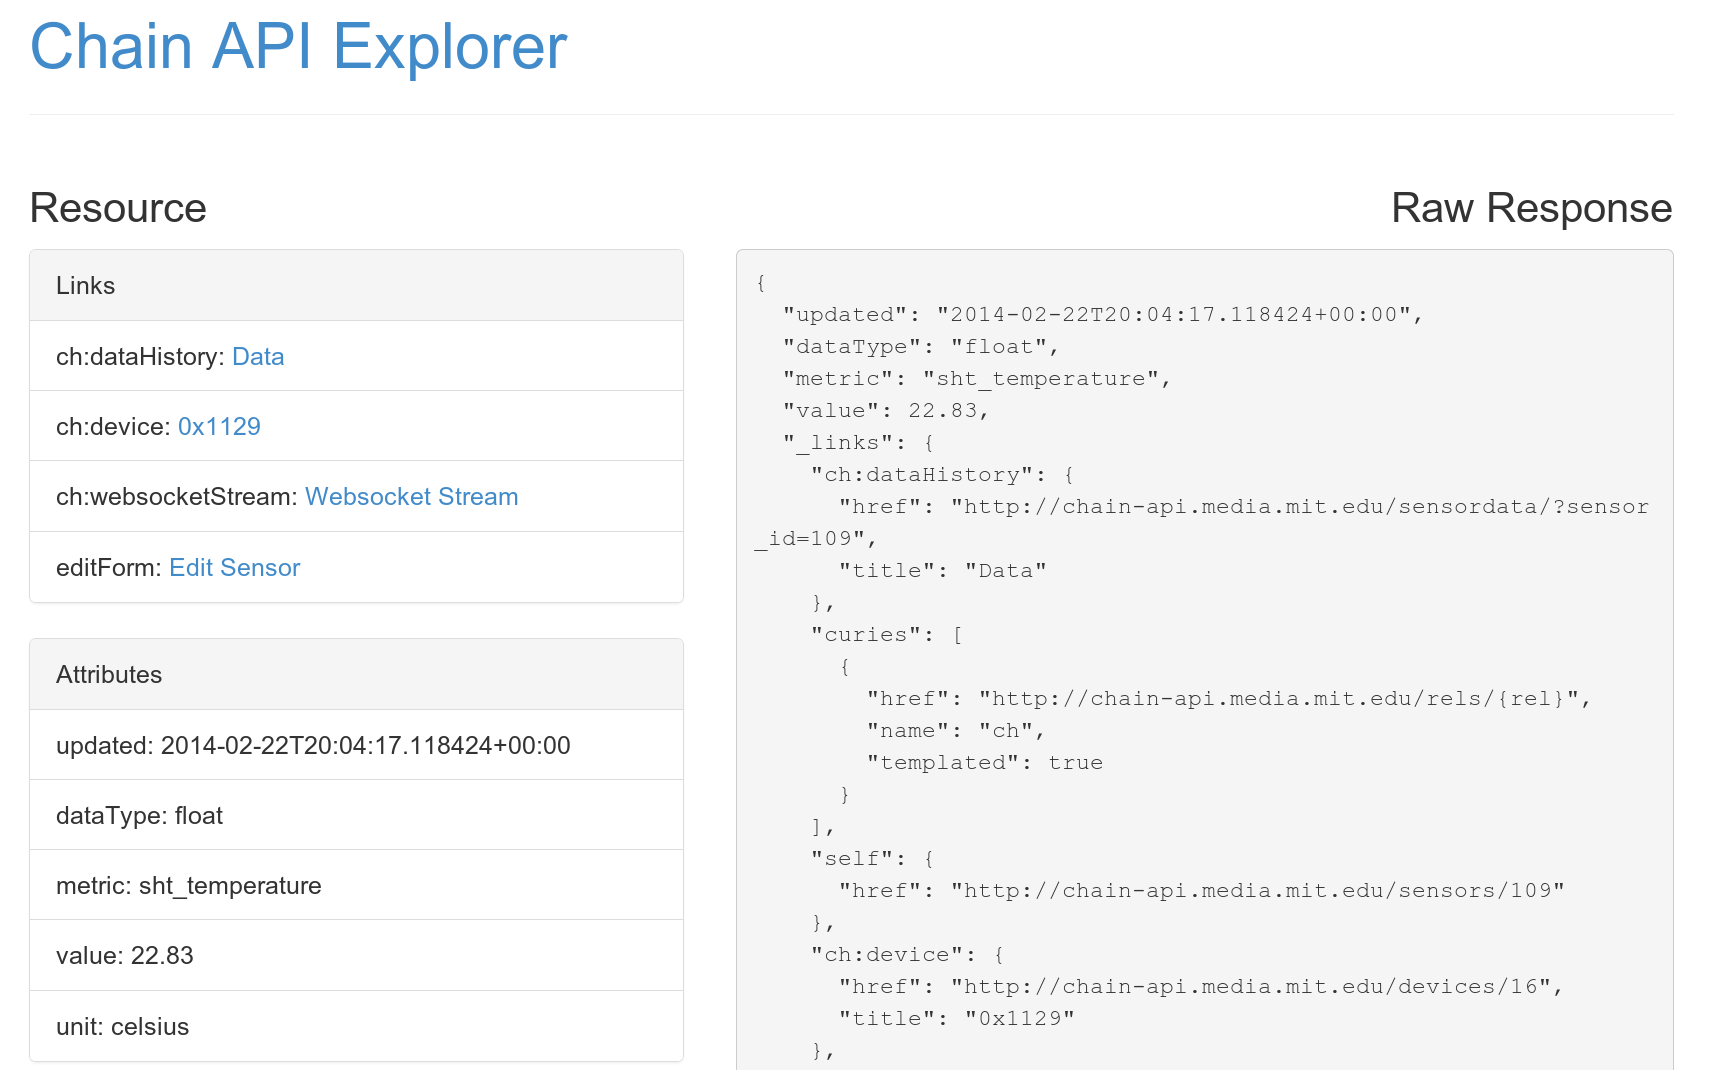
\includegraphics[width=8.45cm, frame]{chain_explorer2}
    \caption{Chain API Explorer}
    \label{chain_explorer}
\end{figure}

To assist developers building applications on top of ChainAPI, we have
developed a human-facing interface with HTML, CSS, and Javascript that can be
viewed through a standard web browser, as seen in Figure \ref{chain_explorer}.
Through this interface developers can familiarize themselves with the ChainAPI
interface before they start their client application, or to evaluate ChainAPI
for their application. For each request, we display the raw JSON of the
response on the right side. On the left we display a more user-friendly and
interactive rendering of the raw data.

Our HTML interface has the following capabilities

\begin{tightenumerate}
    \item Display resource attributes
    \item Display links as clickable HTML links
    \item Create and \texttt{POST} an HTML form from a JSON-Schema
    \item Plot time-series data on a graph
\end{tightenumerate}

Capabilities 1-3 are enough to enable a user to fully interact with the API
without any specialized code on the client side. Plotting time-series data is a
convenience to help visualize the data, but is not a core requirement of client
libraries. As new features and capabilities are added to the server, they
automatically become available in the client interface with no client-side code
changes.

\section{Implementation}

Our current implementation of the ChainAPI server is written in Python. We use
the Django\footnote{https://www.djangoproject.com/} web framework for the
request/response API and database interactions and a separate process built on
the Flask\footnote{http://flask.pocoo.org/} web framework for managing the
WebSocket connections. The two processes communicate with each other through a
ZMQ socket for event notification. We are currently using the
PostgreSQL\footnote{http://www.postgresql.org/} relational database. Nginx acts
as a reverse-proxy server to dispatch standard HTTP and also WebSocket
connections to the application servers.


\section{Case Study:\\Tidmarsh Living Observatory}

The Tidmarsh Living Observatory project\footnote{http://tidmarshfarms.com/} is
a sensor deployment at a former cranberry bog in southern Massachusetts that is
currently undergoing a restoration to a natural wetland. There are currently 15
sensors nodes deployed, each sensing temperature, humidity, barometric
pressure, and ambient light. Each node is powered by 3 AA batteries, with an
expected battery life of approximately 2 years. Approximately 150 additional
nodes will be installed in the coming months. Figure \ref{tidmarsh_arch} shows
an overview of the Tidmarsh architecture.

\begin{figure}
    \centering
    % load the library when editing in QTikZ, comment out for inclusion in the paper
%\usetikzlibrary{positioning}
\begin{tikzpicture}[
	sensornode/.style={
		shape=rectangle,
		draw,
		minimum size=10mm,
		rounded corners,
	},
	gateway/.style={
		shape=rectangle,
		draw,
		rounded corners,
		minimum width=25mm,
		minimum height=10mm,
	},
	server/.style={
		shape=rectangle,
		draw,
		rounded corners,
		minimum width=25mm,
		minimum height=10mm,
		text width=22mm,
		align=center,
	},
	client/.style={
		shape=circle,
		draw
	},
	>=stealth,
	->,
	thick,
	font=\footnotesize,
	node distance=7mm,
]
% draw the bounding rectangle
%\draw (0,0) rectangle (8.45, 10);

\node (n4) [sensornode] at (2.5,1) {Node};
\node (n5) [sensornode, right=of n4] {Node};
\node (n7) [sensornode, above=of n4] {Node};
\node (n6) [sensornode, left=of n7] {Node};
\node (n8) [sensornode, right=of n7] {Node};
\node (gateway) [gateway, above=of n7] {TCP/IP Gateway};
\node (zmq server) [server, above=of gateway] {Binary $\to$ JSON Translator};
\node (zmq json server) [server, above=of zmq server] {ZMQ $\to$ ChainAPI\\Bridge};

\node (client1)[client, right=of zmq json server] {Client};
\node (client2)[client, right=of client1] {Client};
\node (client3)[client, below=of client2] {Client};
\node (chain server) [server, above =of client1, yshift=10] {ChainAPI Server};

\draw[dashed] (n4) -- (n7);
\draw[dashed] (n5) -- node[right] {Atmel LWM (802.15.4)}(n8);
\draw[dashed] (n6) -- (gateway);
\draw[dashed] (n7) -- (gateway);
\draw[dashed] (n8) -- (gateway);

\draw (gateway) -- node[right] {ZMQ (binary)} (zmq server);
\draw (zmq server) -- node[right] {ZMQ (JSON)} (zmq json server);
\draw (zmq json server) -- node[left] {HTTP} (chain server);
\draw[<->] (client1) -- (chain server);
\draw[<->] (client2) -- node[right, text width=2cm, yshift=1.5mm] {HTTP, \\WebSockets} (chain server);
\draw[<->] (client3) -- (chain server);
\end{tikzpicture}

    \caption{Tidmarsh Architecture}
    \label{tidmarsh_arch}
\end{figure}

\subsection{Sensor Infrastructure}

One of the goals of ChainAPI is to accomodate a wide variety of heterogeneous
underlying sensor systems and provide easy integration. In the case of Tidmarsh
there was an existing sensor installation that exposed the sensor data via
ZMQ\footnote{http://zeromq.org/}.The sensors communicate with a base station
using Atmel's Lightweight Mesh protocol over 802.15.4. Nodes not within direct
communication range of the base station can route messages through
solar-powered router nodes, which are also collecting data. The base station
serves as the TCP/IP Gateway, which receives the RF messages and sends them
over WiFi to  server via ZMQ. The message payloads are left in their binary
format and they are received by the Binary to JSON translator, which parses the
binary messages and generates JSON representations of the data. The Binary to
JSON translator acts as a ZMQ server, and the JSON messages are sent to any
connected clients.

\subsection{ChainAPI Representation}

Each sensor node is a Device in the ChainAPI ontology.

\subsection{Client Behavior}

We developed a client built on the Unity3D game
engine\footnote{http://unity3d.com/} to explore and experience the data from
the sensor network.

\section{Conclusion}
And here we conclude, with some stirring remarks.

%ACKNOWLEDGMENTS are optional
\section{Acknowledgments}
We would like to thank Cisco Systems, who provides partial funding for this
project.

% The following two commands are all you need in the
% initial runs of your .tex file to
% produce the bibliography for the citations in your paper.
\bibliographystyle{abbrv}
\bibliography{refs}  % sigproc.bib is the name of the Bibliography in this case
%
% ACM needs 'a single self-contained file'! For final submission paste the contents
% of refs.bbl here.
%
\end{document}
